\section{Hardware}
I dette afsnit beskrives alle de hardware implementeringer vi har foretaget i projektet. Dette involverer alle sensorer samt generel opbygning af print til bilen.

\subsection{Accellerometer}

\begin{wrapfigure}{r}{4cm}
	\begin{minipage}{.3\textwidth}\centering
		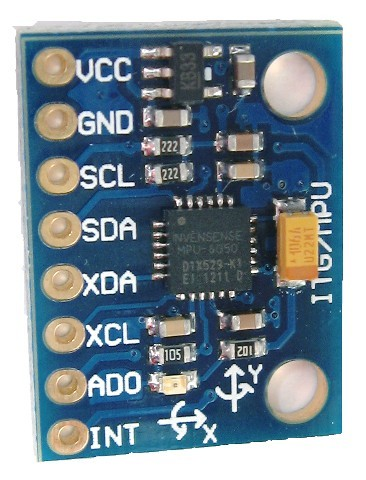
\includegraphics[scale=0.2]{Billeder/mpu-6050.jpg}
		\caption{MPU-6050\\Breakout Board}
		\label{fig:MPU-6050-Breakout}
	\end{minipage}
\end{wrapfigure}

Til projektet er der valgt at bruge en gyro, til at bestemme hvilken type sving bilen er i. Til projektet var der mulighed for at få udleveret et analogt og et digitalt accelramometer.
\\Det digitale var et LIS35DE, som kan måle \textpm 2G eller \textpm 8G på 3 akser, og kan lave målinger op til 400 gange i sekundet.\ Det analoge var et MMA1270KEG med kun en akse, der kan måle op til \textpm 2,5G. Den akse det kan måle på ligger vinkelret på printet, som chippen bliver placeret på.
\linebreak

I gruppen havde vi en MPU-6050 tilrådighed, som har 3 akset accelramometer, som sender 16bit data ud for hver akse, det er her muligt at sætte følsomheden til: \textpm 2G, 4G, 8G eller 16G. Men udover at have et accelramometer så har den også en 3 akset gyro, som vi i gruppen havde en ide om, kunne gøre det nemmere at se forskel på, om det er et stort sving eller  lille sving. I gruppen valgte vi at bruge MPU-6050, da det gav os mulighed for at bruge både gyro og accelramometer, så vi ikke skulle lave noget om, hvis vi ikke fik nogle brugbare værdier fra gyroen.
\linebreak

\subsubsection{Logic level shifter}

\begin{figure}[h]\centering
	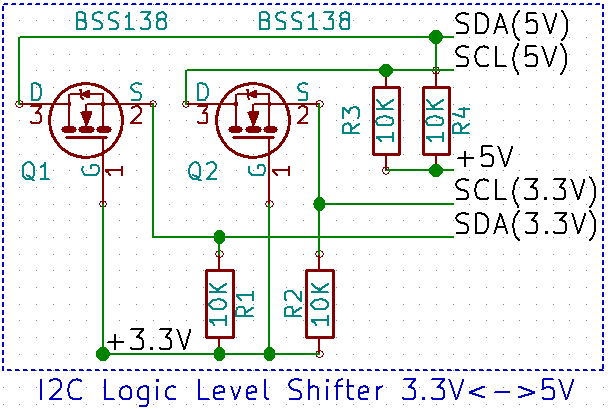
\includegraphics[scale=0.4]{Billeder/LogicLevelShifter.PNG}
	\caption{Logic level shifter}
	\label{fig:LogiLevelShifter}
\end{figure}

MPU-6050 breakout boardet fungerer kun med 3,3V, og der er derfor behov for en logic level shifter, som skal omsætte 3,3V I$^{\text{2}}$C til 5V I$^{\text{2}}$C. I$^{\text{2}}$C fungere på den måde, at linjerne altid er trukket til 5V eller 3,3V ved hjælp af pull up modstande, og når der så bliver sendt data, så bliver linjen trukket til ground for et digitalet 1.
På figur \ref{fig:LogiLevelShifter} kan man se de 2 5V pull up modtstande, de 2 3,3V pull up modstande og så de 2 MOSFET´s som får 3,3V


\subsection{Lap sensor}

Til at holde øje med når bilen krydsede målstregen, faldt valget på en CNY70 optisk sensor. Den består af en infrarød lysdiode og en phototransistor bygget ind i samme hus. Dioden sender hele tiden infrarødt lys ud gennem et lille vindue, og hvis der er en flade tæt på til at reflektere lyset, vil det blive opfanget af phototransistoren, der sidder ved siden af dioden bag et lysfilter. Mængden af lys der bliver reflekteret tilbage afhænger af afstanden til fladen, og typen af materiale der er på overfladen - en hvidt malet streg vil for eksempel reflektere mere lys tilbage end en sort materet overflade.

For at gøre signalet fra sensoren brugbart for microcontrolleren, ville vi bruge en komparator til at digitalisere outputtet. Oprindeligt var planen at bruge en LM311 komparator, men det viste sig at den interne komparator i microcontrolleren, lige så nemt kunne bruges til det formål, og så ville der også skæres ned på antallet af eksterne komponenter og derved mindske pladsforbruget på vores print. En anden fordel ved at bruge den interne komparator, er at det bliver muligt at bruge den interne spændingsreference på 2.56 V som input til komparatoren. Så er det bare et spørgsmål om at dimensionere outputtet fra CNY70 sensoren med en modstand, så spændingen, der kommer fra den sorte overflade på banen, ligger under 2.56V, og spændingen fra den hvide målstreg ligger over. Microcontrolleren aflæser komparatoren ved at se på outputtet fra den, og det kan sættes op, så den sender et interrupt, når der kommer en rising eller falling edge, eller når outputtet skifter tilstand. Med denne løsning bruges der kun tre eksterne komponenter - en modstand hver til henholdsvis lysdioden og phototransistoren samt CNY70 sensoren. Modstanden til lysdioden blev sat til 150 ohm, så der løber godt 30 mA i det kredsløb. For at opfylde spændingskravene til komparatoren blev der brugt en 22 kilo-ohms modstand - det gav en spænding på banen omkring 0.8 V og en spænding på målstregen på ca 4.5 V.

\subsection{Tachometer}

Til at måle omdrejningshastigheden på bilen, samt at opfylde kravet om en elektrofysisk sensor/aktuator, blev der valgt en analog hall sensor som monteredes på motoren. Sensoren har tre ben - et til 5 V, et til stel og et output. Outputtet ligger og svinger omkring 2.5 V og ændrer sig i positiv eller negativ retning alt afhængigt af, hvordan den magnetiske flux ændrer sig i nærheden af sensoren. Når motoren kører, vil man på hall sensorens output, så kunne måle, når polerne passerer tæt forbi sensoren. Det giver et svagt og noget støjet signal, der skal behandles for, at microcontrolleren kan bruge det til noget. Det rå signal havde en peak-to-peak spænding på 100-200 mV, så det var ret vigtigt først at få det forstærket op. Det havde også den tilføjede bonus at skære noget af den mere højfrekvente støj fra, fordi den forstærker vi valgte, en instrumenteringsforstærker AD623, havde en knækfrekvens på godt og vel 90 kHz, under de forhold vi arbejdede under. 

\begin{figure}[h]

	\centering
		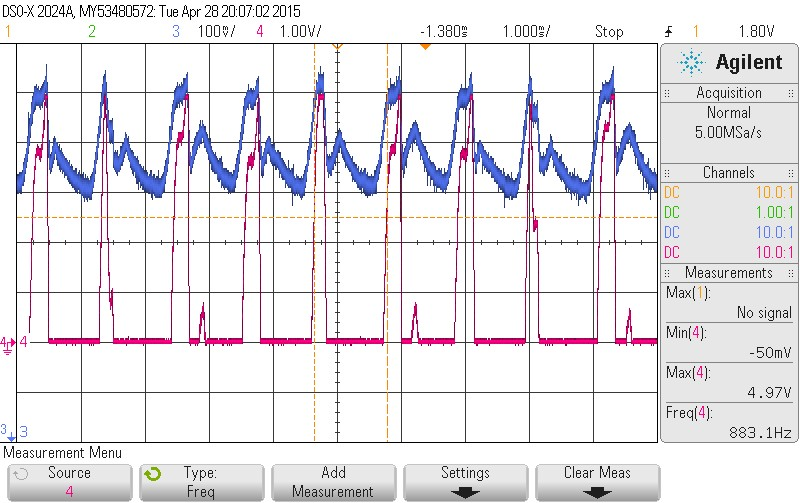
\includegraphics[scale=0.4]{Billeder/Signal1.jpg}
	\caption{Her ses signalet fra hall sensoren før (blå) og efter (lyserød), det er blevet behandlet af forstærkeren.}
	\label{fig:Signal1}
	
\end{figure}

Ud fra de første målinger, viste det sig at den lave del af signalet, var meget støjfyldt og svær at behandle, så vi valgte at skære den del af signalet fra med et offset på forstærkeren se figur \ref{fig:Signal1}. Offsettet blev styret af et potentiometer, der blev brugt som en slags justerbar referencespænding.

\begin{figure}[h]

	\centering
		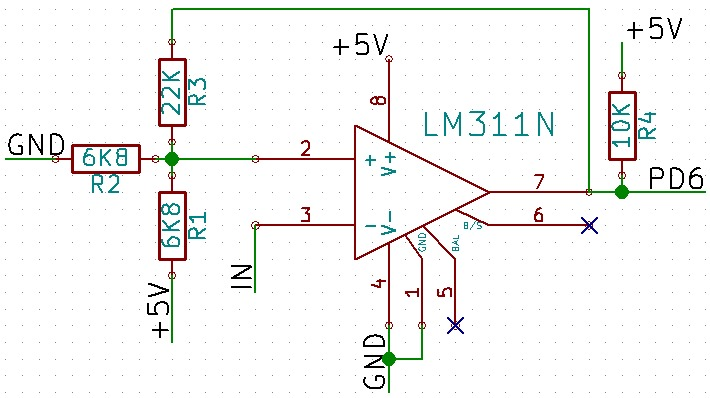
\includegraphics[scale=0.3]{Billeder/Schmitt.jpg}
	\caption{Diagram over schmitt trigger kredsløbet.}
	\label{fig:Schmitt}
	
\end{figure}

For at digitalisere signalet, så microcontrolleren kunne behandle det, blev der brugt en komparator - denne gang som en schmitt trigger for at formindske fejl. Det var ikke nødvendigt at designe spændingstærsklerne på schmitt triggeren så præcist. De skulle bare ligge relativt langt fra hinanden, så eventuel støj ikke kunne få den til at skifte tilstand utilsigtet. Ud fra  målinger med oscilloskop viste det sig, at et spænd på over 0.5 V var rigeligt til at forhindre støj i at få schmitt triggeren til at skifte tilstand.

\begin{equation}
V_{TL} = \dfrac{R_{2}||R_{3}}{R_{2}||R_{3}+R_{1}} \cdot 5V
\label{eq:Vtl}
\end{equation}


\begin{equation}
V_{TH} = \dfrac{R_{2}}{R_{2}+R_{1}||(R_{3}+R_{4})} \cdot 5V
\label{eq:Vth}
\end{equation}



Til at beregne spændingstærsklerne skal man finde spændingen på det ikke-inverterende ben, når komparatoren er åben, og når den er lukket. Så ender man med to ligninger med to ubekendte, hvis man fastsætter to af modstandene og spændingstærsklerne på forhånd. Modstandsværdierne blev dikteret af udvalget på komponentlageret, og ved hjælp af ligning \eqref{eq:Vtl} og \eqref{eq:Vth} designede vi spændingstærskler på henholdsvis 2.2 V og 2.8 V. 

\subsection{Bremse}
\label{sec:Bremse}

For at bremse bilen kortsluttes motorterminalerne. En kortslutning bremser motoren ved at lade et magnetfelt, der modsætter sig motorens bevægelse, blive induceret i spolerne. Hvis kortslutningen ikke er til stede, kan der ikke løbe nogen strøm og derfor heller ikke dannes noget modsatrettet magnetfelt. Selve kortslutningen bliver udført af 5 volts relæ, der bliver styret af en MOSFET forbundet til et IO-ben på microcontrolleren. Se figur \ref{fig:Schematic}. 

\subsection{Elektromagnet}
I dette projekt har vi valgt at se på en elektromaget, for at se om det kunne svare sig at implementere en elektromagnet, for at kunne bremse/holde bilen på Banen.\\
En elektromagnet er en spole med tilhørende kerne som laver et magnetiskfelt ved at sende strøm igennem en spole. Der er flere forskellige måder, man kan påvirker dette felt på for eksempel ved at sende en kraftigere strøm igennem spolen eller have flere vindinger på spolen. Du kan også ændre den styrke ved at tilføje en kerne til elektromagneten, Det denne kerne gør at den magnetiske felter nemmer, kan trænge igennem kernen, end de kan i luft. Disse kerner bliver oftest lavet af jern.
Når elektromagneten ikke er tændt vil alle de forskellige magnetiske felter være spredt ud i alle retninger, og når du så tilføjer en strøm vi de all sammen blive ensrettet, og derved bliver elektromagneten stærkere.

Disse elektromagnet bliver brugt mange forskellige steder, så som i industrien, hvor de bliver brugt til løfte meget tunge magnetiske ting, som for eksemple biler.
 
For at regne på en elektromagnet bliver designet valgt således, at man regner magneten, som et stykke. Hvor vi så regner på den magnetiske energi i forhold til, hvor langt de er væk for hinanden. Den vil være U-formet med en strøm I og N antal vindinger, samt en længde L igennem elektromagneten og banen.


Ud fra amperes lov fås følgende


$$H_j \cdot L+2 \cdot H_s \cdot x = N \cdot I$$

Hvor dette er gældende

$$H_j = \dfrac{B_j}{\mu_0 \cdot K_m}, H_s = \dfrac{B_s}{\mu_0}$$

Her er $B_j$ det magnetiske felt for kernen, og $B_s$ er det magnetiske felt for det tommerum mellem banen og magneten. $H_j$ og $H_s$ er de til hørende H-felter. Til sidste har vi fejlen som i det enklte materiale $K_m$

Da vi går ud fra at der ikke er nogen spredning bliver $B_j = B_s$ og derved får vi dette


$$B_j(x) = \dfrac{\mu_0 \cdot I \cdot N}{(\dfrac{L}{K_m}+2 \cdot x)}$$

Ud fra dette kan vi finde den magnetiske energi og derefter finde kraften ved $F_{mag} = -\dfrac{dU_B}{dx}$

så får vi følgende udtryk, som bruges til at beregne kraften af en U formet elektromagnet

\begin{equation}
F_{mag} = - \dfrac{B_j^2}{2 \cdot \mu_0} \cdot A_j
\end{equation}
Hvor vi går ud fra at fejlen $\dfrac{L}{K_m}+2 \cdot x = 2 \cdot x$ hvis $K_m$ er meget stor, og x er meget lille, som i de fleste tilfælde er rigtigt, da kernen af elektromagnet vil være lavet af jern og da kraften skal være så stor som mulig, vil den også være så tæt på banen som mulig.

Vi valgt ikke at gå videre med at bruge en elektromagnet, da vi fandt en anden måde at bremse på som der kan læses om i sektion \ref{sec:Bremse}. Vi kunne se rent visuelt at det ville være svært at implentere elektromagneten, da den ville blive forholdsvis stor, hvis den skulle være effektiv nok. Uf fra den forudsætning at bilen skulle veje, så lidt som mulig og have det lavest mulige tyngdepunkt. 

\pagebreak
\subsection{Print}
Dette afsnit beskriver kort printet som der er blevet lavet til bilen. Vi har lavet det som et skjold der monteres ovenpå bilen i de headers som der allerede er på det print vi har fået udleveret. Figur \ref{fig:Schematic} viser hele det skematiske overblik over printet. Og figur \ref{fig:Print} viser det fremstillede print. Vi har designet det sådan at alle headers sidder så de ikke kommer i kambullage med karrosseriet på bilen.

\begin{figure}[h]
	\centering
		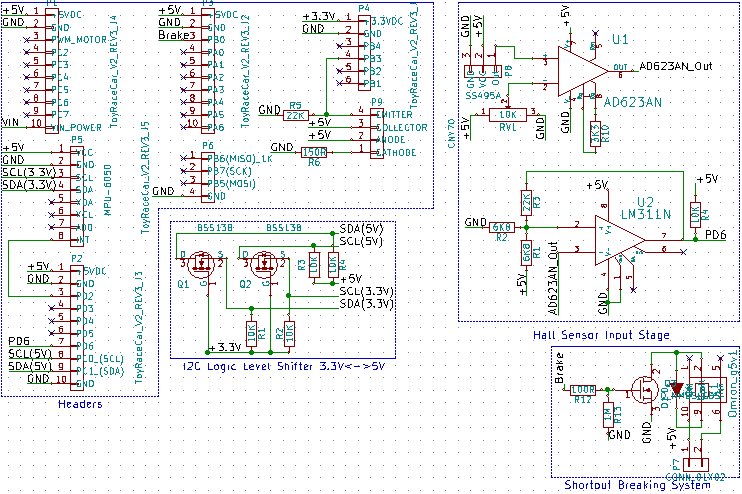
\includegraphics[scale=0.8]{Billeder/Schematic.PNG}
	\caption{Her ses hele schematic til det print der er blevet lavet til bilen. De individuelle dele er beskrevet i de relevante hardware afsnit}
	\label{fig:Schematic}
\end{figure}

\begin{figure}[h!b]
	\centering
		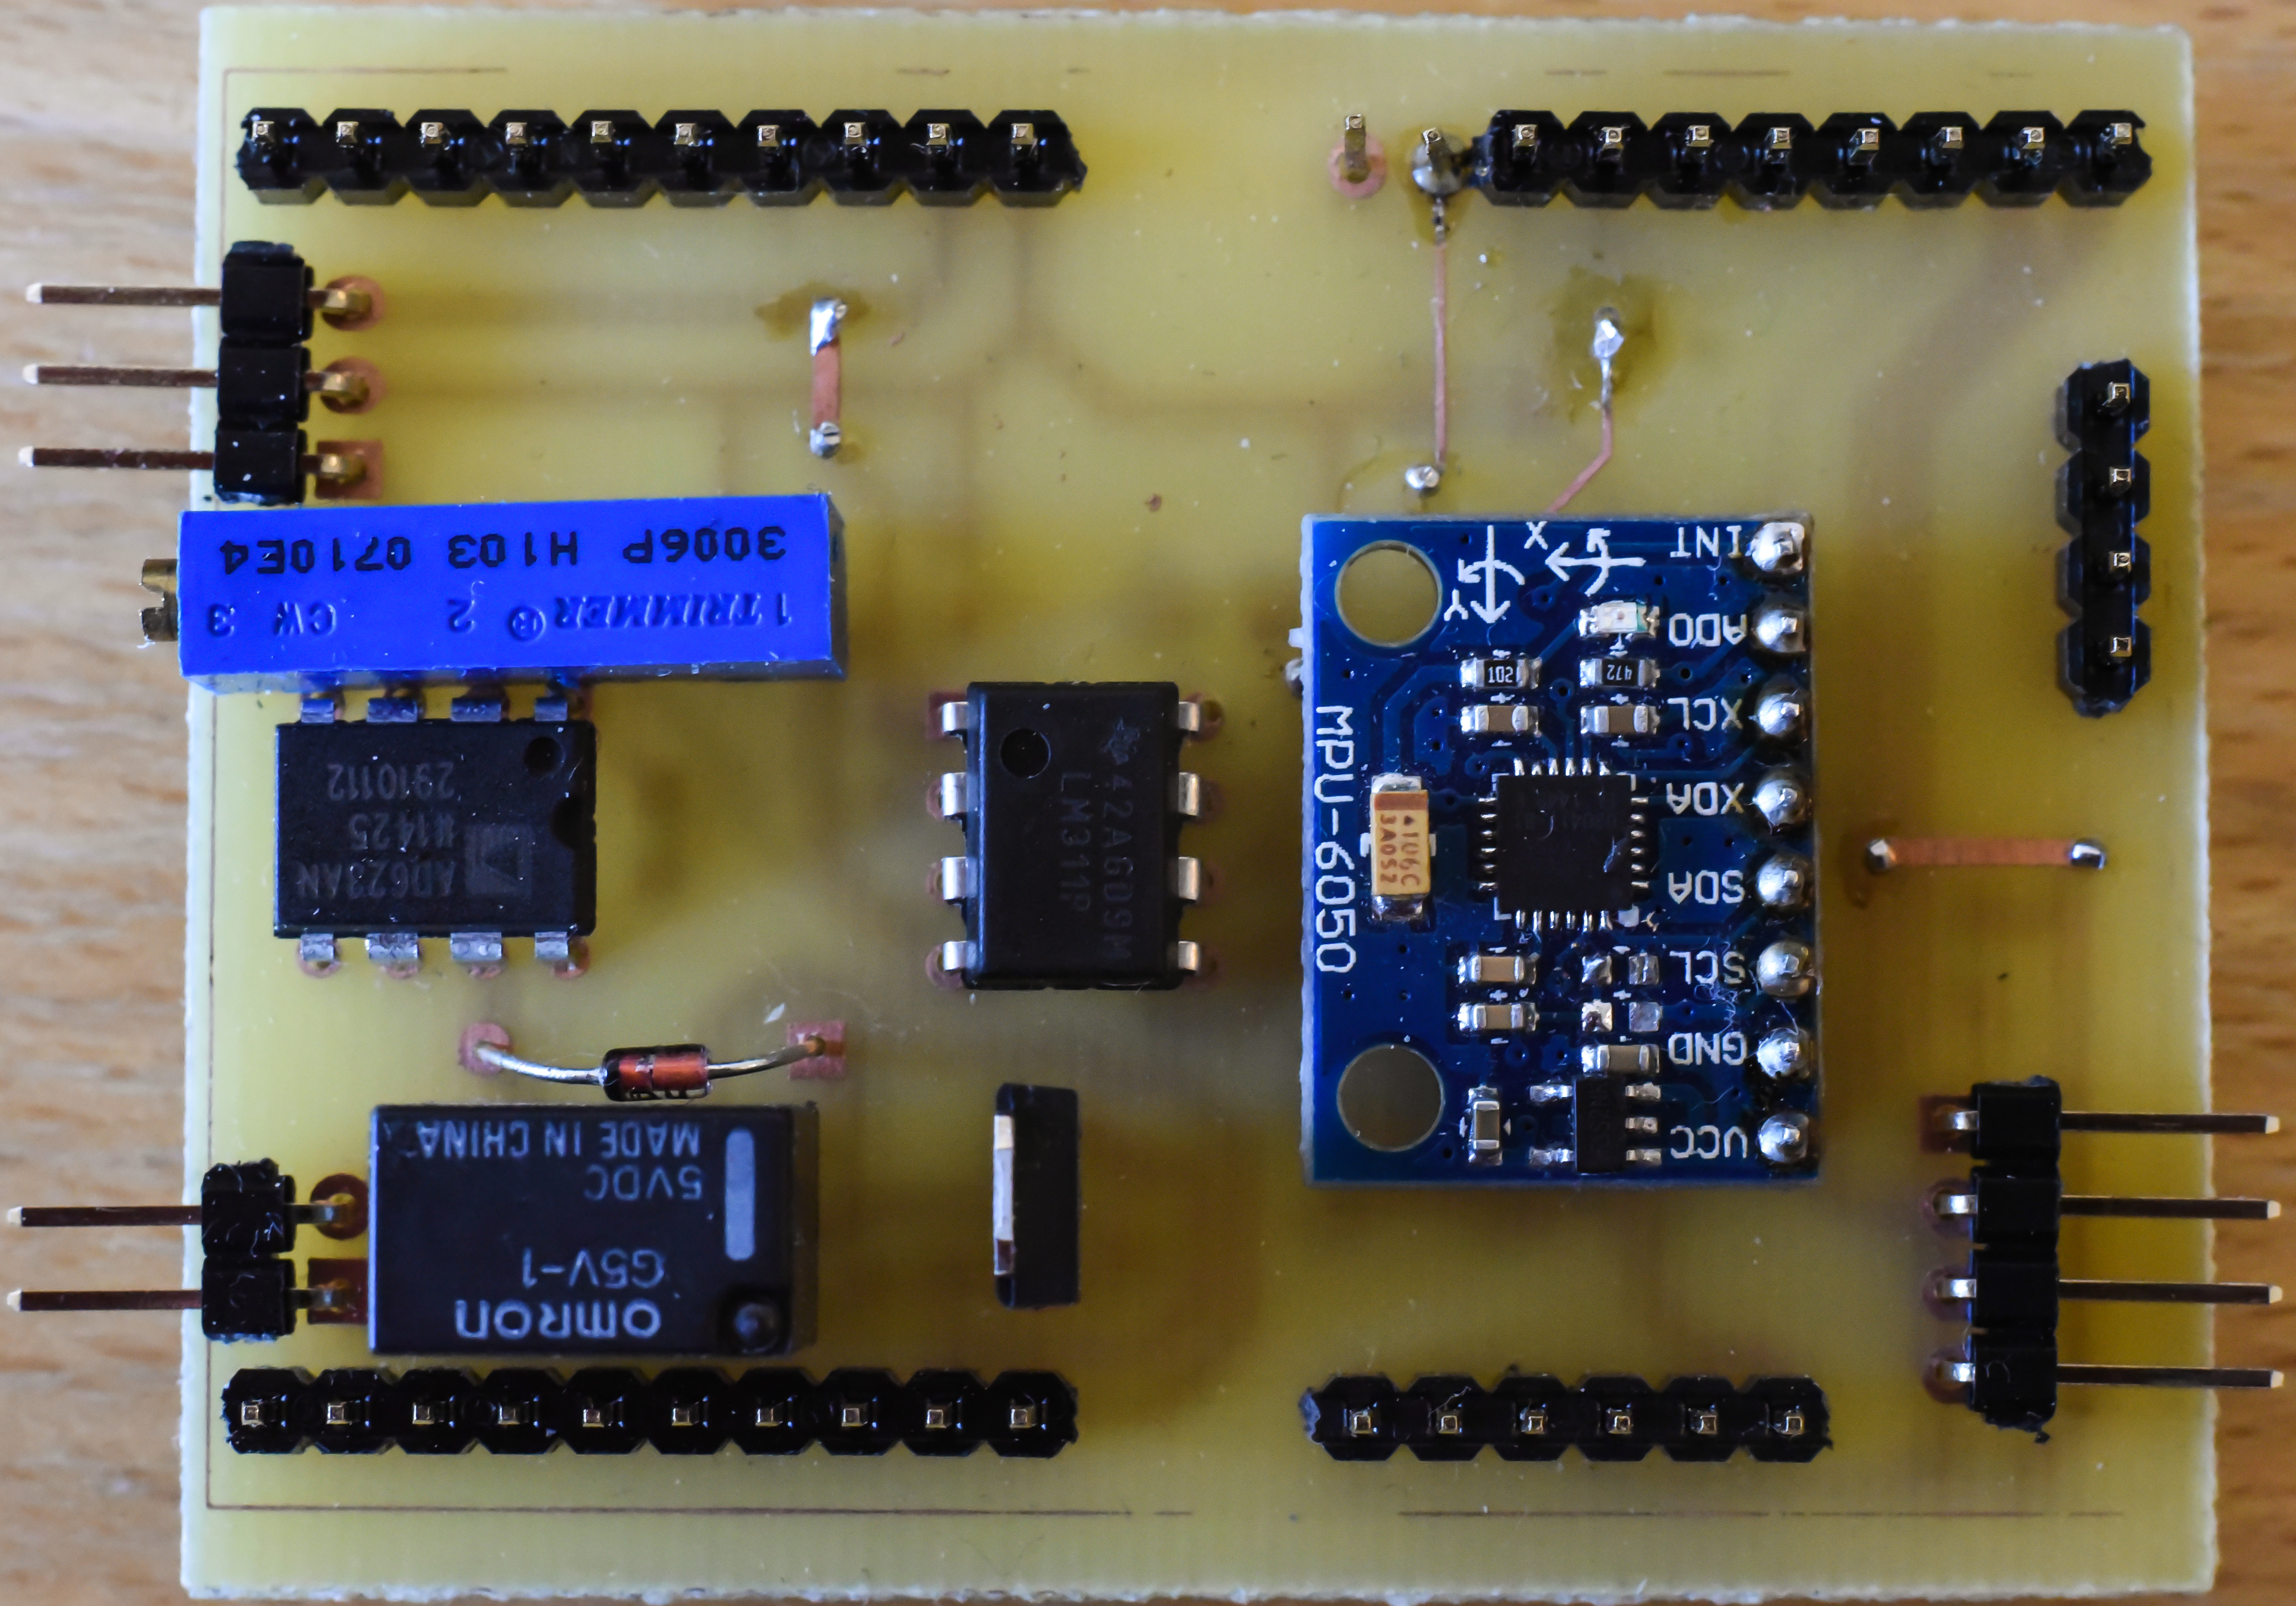
\includegraphics[scale=0.04]{Billeder/Print-top.JPG}
	\caption{Her ses det færdige print}
	\label{fig:Print}
\end{figure}


